\documentclass[../DS04.tex]{subfiles}
\graphicspath{{./figures/}}

\begin{document}

\exercice[40]{Comparaison de deux circuits RLC}
% \subimport{/home/nora/Documents/Enseignement/Prepa/bpep/exercices/DS/comparaison_de_deux_circuits/}{sujet.tex}
\enonce{
	Dans toute la suite du problème, on considère les deux circuits suivants,
	composés d'un résistor de résistance $R=\SI{0,5}{k\ohm}$, d'un condensateur
	de capacité $C=\SI{1,0}{\micro F}$ et d'une bobine d'inductance
	$L=\SI{1,0}{mH}$. Ces composants sont branchés sur un générateur idéal de
	tension de f.e.m. $E$.
	\bigbreak
	On considère de plus que les interrupteurs $K$ sont ouverts lorsque $t<0$ et
	sont fermés à partir de l'instant initial $t=0$. De plus, les condensateurs
	sont initialement déchargés.
	\smallbreak
	\noindent
	\begin{minipage}[t]{.45\linewidth}
		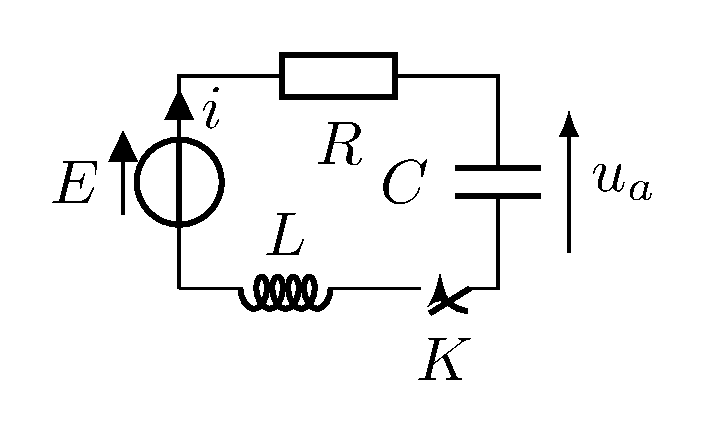
\includegraphics[width=\linewidth]{circuit_serie}
		\captionof{figure}{Circuit A}
	\end{minipage}
	\hfill
	\begin{minipage}[t]{.52\linewidth}
		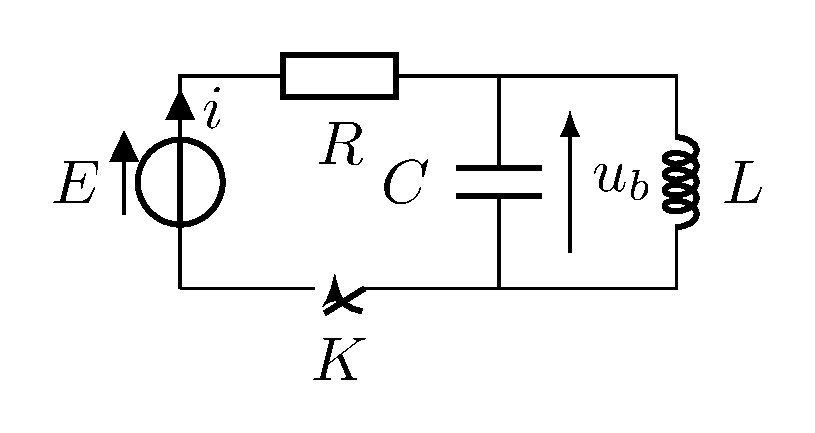
\includegraphics[width=\linewidth]{circuit_para}
		\captionof{figure}{Circuit B}
	\end{minipage}
	\begin{tcb}(odgr){Aide au calcul}
		\vspace{-15pt}
		\begin{gather*}
			\frac{1}{5} = \num{0.2}
			\quad ; \quad
			10^{-1/2} \approx \num{0.32}
			\quad ; \quad
			\frac{1}{6.3} \approx \num{0.16}
			\\
			\sqrt{2} \approx \num{1.414}
		\end{gather*}
	\end{tcb}
}

\subsection{Étude en régime transitoire}

\enonce{
	On considère dans un premier temps le circuit A et on cherche à obtenir
	l'expression de $u_a(t)$
}

\QR[7]{
	Obtenir l'équation dont $u_a$ est solution lorsque $t>0$ et la mettre sous la
  forme
	\begin{equation}
		\label{eq:circuit_1}
		\dv[2]{u_a}{t} + \frac{\w_0}{Q_a} \dv{u_a}{t} + \w_0^2 u_a = \w_0 ^2 E
	\end{equation}
	On veillera on particulier à donner les expressions de  $\w_0$ et $Q_a$, le
	facteur de qualité du circuit A. Réaliser ensuite l'application numérique pour
	$Q_a$.
}{
	Le circuit ne comporte qu'une maille et ne peut donc être simplifié, on
	applique alors la loi des mailles
	\[
		E = R i + u_a + L \dv{i}{t}
		\Rightarrow
		E = RC \dv{u_a}{t} + u_a + LC \dv[2]{u_a}{t} \Rightarrow
		\boxed{ \dv[2]{u_a}{t} + \frac{R}{L} \dv{u_a}{t} + \frac{1}{LC} u_a =
			\frac{1}{LC} E}
	\]
	On en déduit par identification que $\boxed{\w_0 = 1/\sqrt{LC}}$ puis après
	calcul que $\boxed{Q_a = \frac{1}{R}\sqrt{\frac{L}{C}} \approx 0,063}$.
}

\QR[5]{
	Obtenir l'équation dont $u_b$ est solution lorsque $t>0$ et la mettre sous la
	forme
	\begin{equation}
		\label{eq:circuit_2}
		\dv[2]{u_b}{t} + \frac{\w_0}{Q_b} \dv{u_b}{t} + \w_0^2 u_b = 0
	\end{equation}
	On veillera on particulier à vérifier que l'expression de $\w_0$ est
	compatible avec celle obtenue pour le circuit A et on vérifiera que
	$Q_b = 1/Q_a$. Réaliser ensuite l'application numérique pour $Q_b$.
}{
	Aucune simplification ne peut être réalisée pour ce circuit, on considère
	alors la loi des noeuds et la loi des mailles (petite maille de gauche)~:
	\[
		i = C \dv{u_b}{t} +i_L
		\Rightarrow
		\dv{i}{t} = C \dv[2]{u_b}{t} + u_b/L
		\qet
		E = Ri + u_b
	\]
	En combinant ces equations, on obtient après avoir dérivé la loi des mailles
	\[
		0 = RC \dv[2]{u_b}{t} + \frac{R}{L} u_b + \dv{u_b}{t}
		\Rightarrow
		\boxed{ \dv[2]{u_b}{t} + \frac{1}{RC} \dv{u_b}{t} + \frac{1}{LC} u_b = 0}
	\]
	On obtient alors par identification $\w_0 = 1/\sqrt{LC}$. Cette expression est
	bien identique à celle obtenue pour le circuit A d'où le même nom. De plus,
	on trouve après calcul que $Q_b = R\sqrt{C/L}$. On en déduit que $Q_b = 1/Q_a$, soit
	\[
		\xul{Q_b \approx 16}
	\]
}

\subsection{Etude en régime sinusoïdal forcé}

\enonce{
	On remplace maintenant le générateur de f.e.m. $E$ par un générateur délivrant
	une tension sinusoïdale $e(t) = E \cos(\w t)$ avec $\w$, une pulsation pouvant
	être modifiée. Dans toute la suite, on notera $\Uu$, l'amplitude complexe
	associée à la tension $u(t)$ en régime sinusoïdal forcé telle que $u(t) = \Re
		(\Uu \exr^{\jwt}) = \Re(\uu(t))$ avec $\jj$, le nombre complexe de module
	unité et d'argument $+\pi/2$ puis $x = \w/\w_0$, la pulsation réduite
	identique aux deux circuits.
	\par
	On considère de plus que l'interrupteur $K$ est remplacé par un fil.
}

\subsubsection{Etude du circuit A}

\QR[2]{
	En partant de l'équation (\ref{eq:circuit_1}), dont on adaptera le second
	membre en remplaçant $E$ par $E\cos(\w t)$, montrer que
	\[
		\Uu_a = \frac{E}{1-x^2 + \jj  \frac{x}{Q_a} }
	\]
}{
	On a donc
	\[
		\dv[2]{u_a}{t} + \frac{\w_0}{Q_a} \dv{u}{t} + \w_0^2 u_a =
		\w_0 ^2 E \cos(\w t)
		\Rightarrow
		\uu(t) \pa{ -\w^2 + \jw \frac{\w_0}{Q_a} + \w_0^2} = \w_0^2 E e^{\jw t}
	\]
	On simplifie alors par les exponentielles complexes et on isole $\Uu_a$~:
	\[
		\Uu_a = \frac{ \w_0^2 E}{\w_0^2-\w^2 + \jj  \frac{\w \w_0}{Q_a} } =
		\frac{ E}{1-x^2 + \jj  \frac{x}{Q_a}}
	\]
	d'où le résultat.
}

\QR[8]{
	Exprimer alors l'amplitude des oscillations $U_a = \abs{\Uu_a}$. Qu'est-ce
	que la résonance~? Établir une condition sur $Q_a$ pour que cette amplitude
	atteigne la résonance. Cette condition est-elle remplie au regard de la
	valeur de $Q_a$ obtenue dans la première partie du problème~?
}{
	On a
	\[
		U_a = \frac{E}{\sqrt{(1-x^2)^2 + x^2/Q_a^2}}
	\]
	Il y a résonance si l'amplitude réelle passe par un maximum à une pulsation
	non nulle et non infinie. Ici, cela revient à avoir le dénominateur minimal.
	Soit $X = x^2$, et $f(X) = \left(1 - X\right)^2 + \dfrac{X}{Q^2}$, la
	fonction que l'on cherche à minimiser~: on cherche donc quand est-ce que sa
	dérivée est nulle, c'est-à-dire
	\begin{DispWithArrows*}
		f'(X_r) &= 0
		\Arrow{On dérive}
		\\\Lra
		-2 \left( 1-X_r \right) + \frac{1}{Q_a{}^2} &= 0
		\Arrow{On isole}
		\\\Lra
		X_r-1 = - \frac{1}{2Q_a{}^2}
		& \Lra
		X_r = 1 - \frac{1}{2Q_a{}^2}
	\end{DispWithArrows*}
	Et on observe qu'il existe une racine réelle uniquement si $\boxed{Q_a >
  \frac{1}{\sqrt{2}} = \frac{\sqrt{2}}{2}}$ (sinon, racines complexes ou
  pulsation nulle, donc pas résonance).
	\par
	En pratique, on a obtenu $Q_a \approx 0,063 < \frac{\sqrt{2}}{2} \approx
		\num{0.707}$. La courbe ne va donc \textbf{pas passer} par un maximum local.
}

\subsubsection{Etude du circuit B}

\enonce{
	Pour le circuit B, on ne peut appliquer la méthode précédente à partir de
	l'équation $(\ref{eq:circuit_2})$ car on y a dérivé des constantes qu'il
	aurait fallu remplacer par des fonctions harmoniques. On se propose alors de
	débuter une nouvelle étude à partir du circuit electronique.
}

\QR[2]{
	Dessiner la représentation équivalente du circuit B en régime sinusoïdal
	forcé.
}{
	\begin{figure}[htbp]
		\centering
		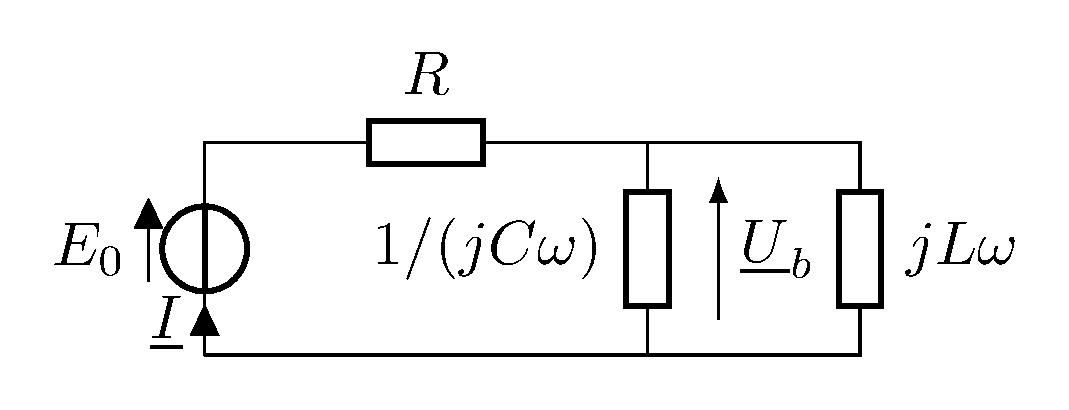
\includegraphics[width=.7\linewidth]{circuit_para_imped}
		\caption{Circuit B en RSF.}
		\label{fig:paraimped}
	\end{figure}
}

\QR[3]{
	Obtenir alors l'expression de $\Uu_b$ en fonction de $x$, $Q_b$ et $E$.
}{
	On peut regrouper la bobine et le condensateur en parallèles
	(impédance $Z\ind{eq}$) puis appliquer un pont diviseur de tension
	\begin{DispWithArrows*}
		\Uu_b           & =
		\frac{\Zu\ind{eq}}{R+\Zu\ind{eq}}E
		\CArrow{$\times \frac{\Yu\ind{eq}}{\Yu\ind{eq}}$}
		\\\Lra
		\Uu_b           & =
		\frac{1}{1+R\Yu\ind{eq}} E
		\Arrow{$\Yu\ind{eq} = \frac{1}{\jlw} + \jcw$}
		\\\Lra
		\Uu_b           & =
		\frac{1}{1+\frac{R}{\jlw} + \jrcw} E =
		\Arrow{$Q_b = R \sqrt{\frac{C}{L}}$}
		\\\Lra
		\Uu_b           & =
		\frac{E}{1 + j R\sqrt{C/L} \pa{ \w \sqrt{LC} - \frac{1}{\w \sqrt{LC}} }}
		\\\Lra
		\Aboxed{  \Uu_b & = \frac{E}{1+jQ_b \pa{x - \frac{1}{x}}} }
	\end{DispWithArrows*}
}

\QR[2]{
	Montrer alors que l'amplitude des oscillations $U_b = \abs{\Uu_b}$ s'exprime
	selon
	\[
		U_b = \frac{E}{\sqrt{1+ Q_b^2 \pa{x-\frac{1}{x}}^2}}
	\]
	puis montrer que cette dernière atteint toujours la résonance, quelle que soit
	la valeur de $Q_b \in \mathbb{R}^+$. Donner la pulsation de résonance.
}{
	On obtient bien l'expression attendue en prenant le module de l'expression précédente
	\[
		\boxed{ U_b = \frac{E}{\sqrt{1+ Q_b^2 \pa{x-\frac{1}{x}}^2}}}
	\]
	L'amplitude passe par un maximum local si le carré de son dénominateur passe
	par un minimum local soit quand $\boxed{x=1}$ et ce, quelque soit $Q_b$. En
	effet, on a $1+ Q_b^2 (x-1/x)^2 \ge 1 + Q_b^2(1-1)^2$ $\forall x >0$.
}

\QR[5]{
Comment se définit la bande passante~? Déterminer l'expression de la largeur
de la bande passante $\Delta \w$ en fonction de $\w_0$ et $Q_b$. On pourra
travailler avec la pulsation réduite ou conserver les pulsations.
}{
C'est l'ensemble des pulsations telles que $U_b (\w) \geq U_{b, \max}/\sqrt{2}$.
On commence par déterminer les pulsations réduites $x_1$ et $x_2$ telles que
$U_b(x_i) = E/\sqrt{2}$~:
\begin{DispWithArrows*}
	1+Q_b^2 (x_i - 1/x_i)^2 &= 2
	\CArrow{$\sqrt{\cdot}$}
	\\\Lra
	Q_b \pa{x_i - \frac{1}{x_i}} &= \pm 1
	\Arrow{$\times x_i$}
	\\\Lra
	Q_b x_i{}^{2} \mp x_i - Q_b &= 0
	\Arrow{Discriminant}
	\\\Ra
	\Delta &= 1 + 4Q_b{}^{2}
	\Arrow{Solutions}
	\\\Ra
	x_{i,\pm,\pm} &= \frac{\pm 1 \pm \sqrt{1+4Q_b{}^{2}}}{2Q_b}
\end{DispWithArrows*}
On obtient alors deux polynômes du second degré (un avec le signe $+$, l'autre
avec le signe $-$). On ne garde que les racines positives, sachant que
$\sqrt{1+4Q_b{}^{2}} > 1$~:
\[
	x_1 = x_{i,-,+} = \frac{1}{2Q_b} \pa{-1 + \sqrt{1+4Q_b{}^{2}}}
	\qet
	x_2 = x_{i,+,+} = \frac{1}{2Q_b} \pa{1 + \sqrt{1+4Q_b{}^{2}}}
\]
puis on obtient
$x_2 - x_1 = 1/Q_b$ soit au final $\boxed{\Delta \w = \w_0 /Q_b}$.
}

\subsubsection{Synthèse}

\QR[6]{
	Quelle est la valeur de $U_a (x=1)$~? La valeur de $U_b (x=1)$~? La valeur de
	$\Delta x$~?
	\bigbreak
	Tracer alors, approximativement mais proprement et sur le même graphique, les
	courbes de $U_a$ et $U_b$ en fonction de $x \in [0,2]$ pour les valeurs des
	facteurs de qualité obtenues dans la première partie. On prendra
	$E=\SI{5}{V}$. On donne $U_a (x=\num{0.74}) = U_b (x=\num{0.74}) \approx
		\SI{0.4}{V}$.
}{
	Pour le circuit A, on observe que $U_a(x=1) = Q_a E \approx \SI{0,32}{V}$ et
	il n'y a pas résonance. Pour le circuit B, on observe une résonance telle que
  $U_b (x=1) = E = \SI{5}{V}$, avec une faible largeur ($\Delta x = 1/Q_b
  \approx 0,063$).
	On obtient alors les courbes suivantes Figure~\ref{fig:gains}.
	\begin{figure}[htbp!]
		\centering
		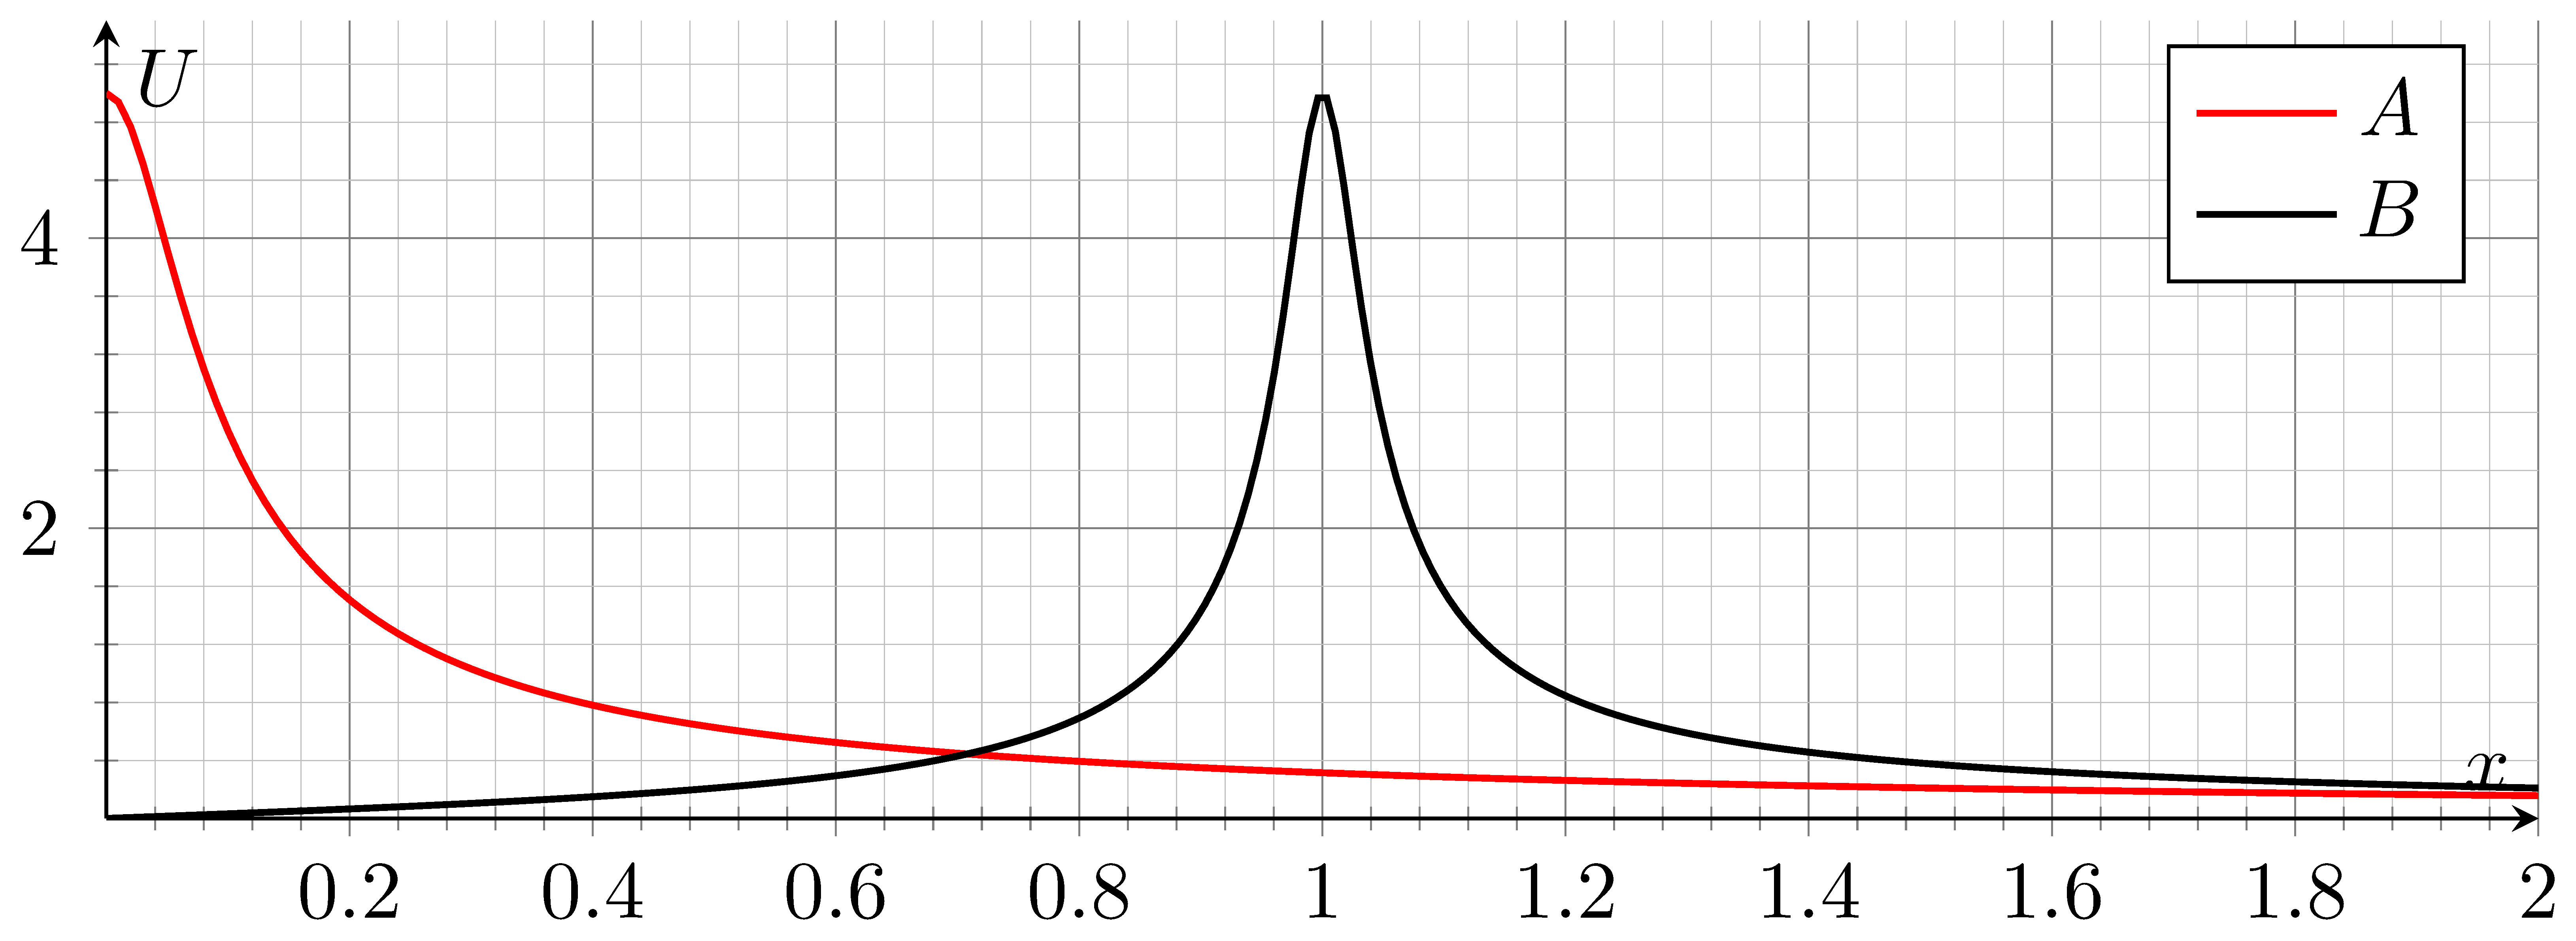
\includegraphics[width=.9\linewidth]{gains_deux_circuits}
		\caption{Gains}
		\label{fig:gains}
	\end{figure}
}

\end{document}
